\thispagestyle{empty}\cleardoublepage
\addcontentsline{toc}{section}{20th Anniversary Papers}
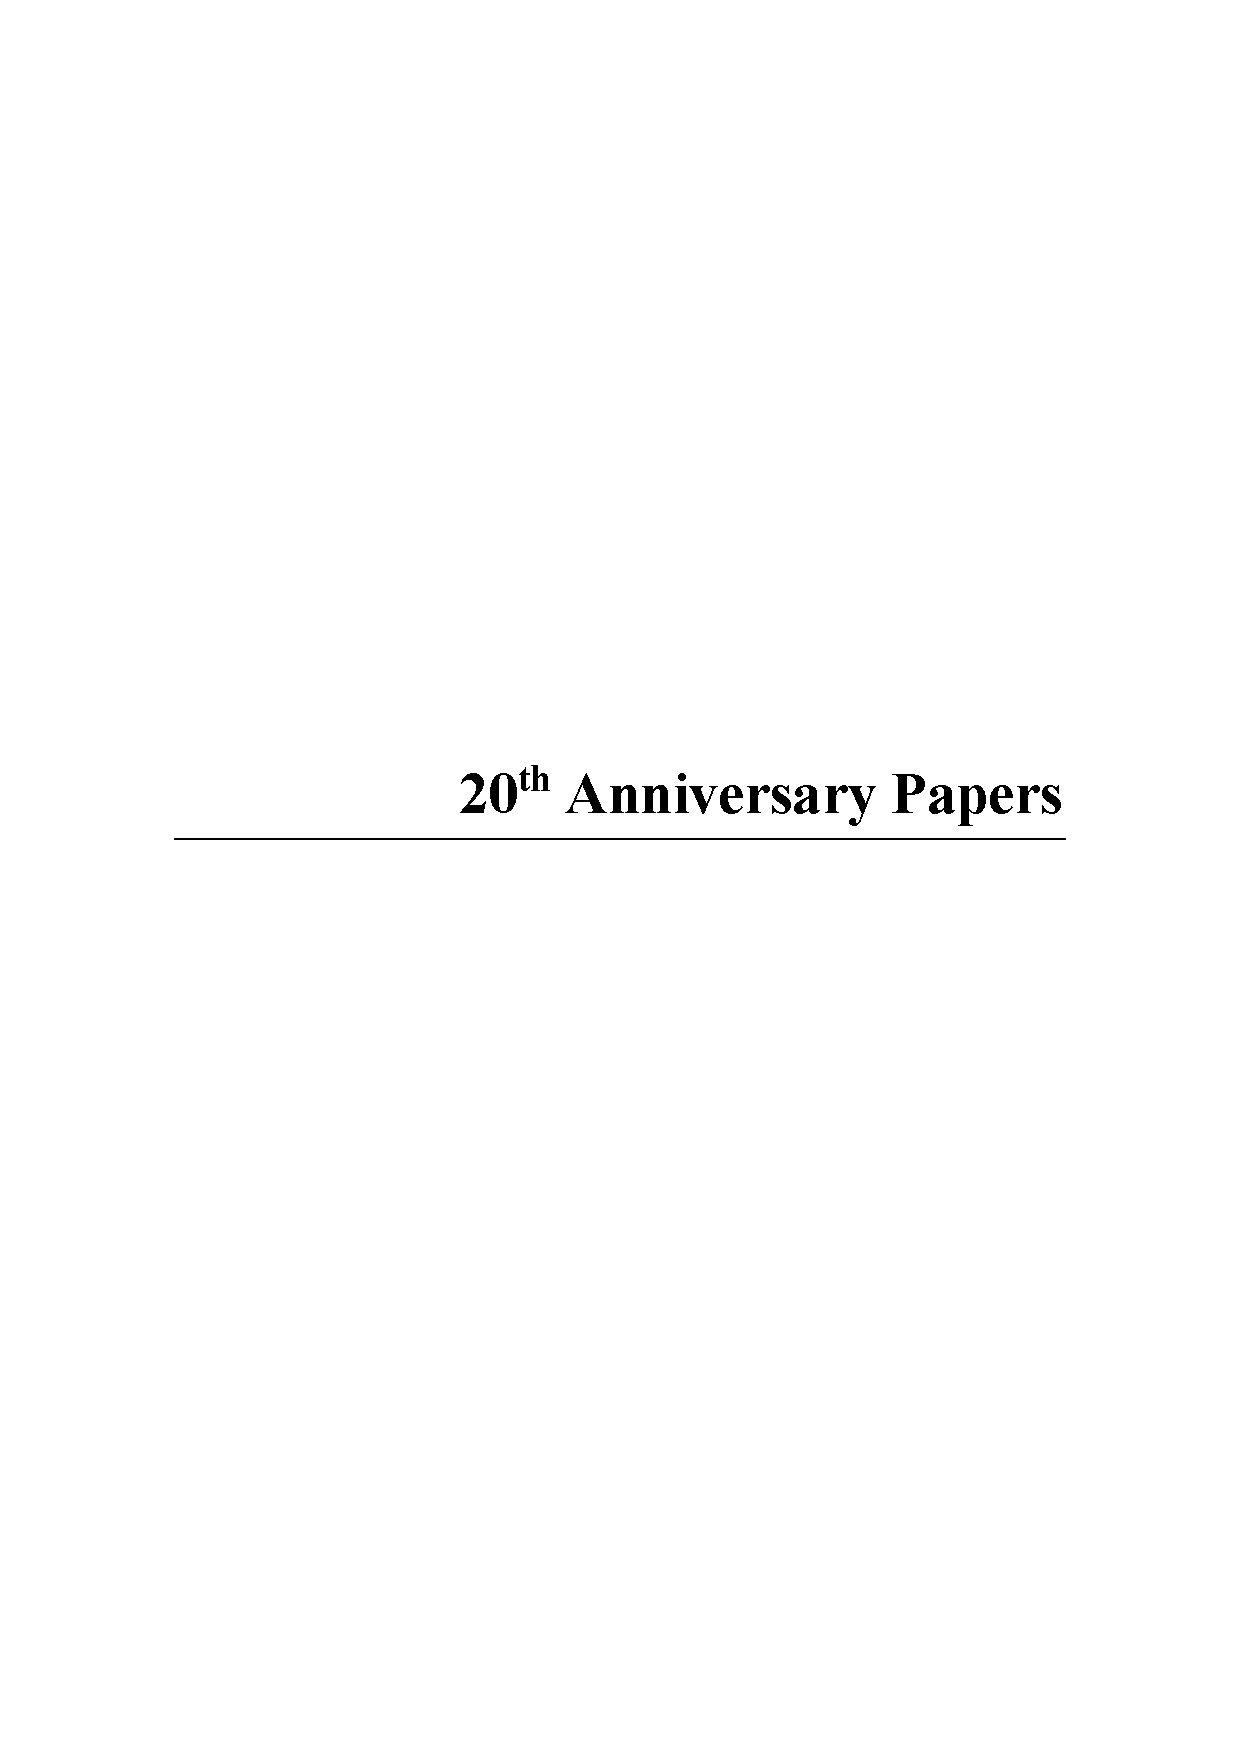
\includepdf[pages=1,pagecommand=\thispagestyle{empty}]{external/12_Sessions.pdf}%
\thispagestyle{empty}\cleardoublepage

\includepaper{Data Usage in MIR: History \& Future Recommendations}{Wenqin Chen, Jessica Keast, Jordan Moody, Corinne Moriarty, Felicia Villalobos, Virtue Winter, Xueqi Zhang, Xuanqi Lyu, Elizabeth Freeman, Jessie Wang, Sherry Cai, Katherine Kinnaird}{articles/paper_239.pdf}
\includepaper{Music Performance Analysis: A Survey}{Alexander Lerch, Claire Arthur, Ashis Pati, Siddharth Gururani}{articles/paper_260.pdf}
\includepaper{Intelligent User Interfaces for Music Discovery: The Past 20 Years and What's to Come}{Peter Knees, Markus Schedl, Masataka Goto}{articles/paper_269.pdf}
\includepaper{20 Years of Automatic Chord Recognition from Audio}{Johan Pauwels, Ken O'Hanlon, Emilia Gomez, Mark B. Sandler}{articles/paper_286.pdf}

\thispagestyle{empty}\cleardoublepage
\addcontentsline{toc}{section}{Session A}
\includepdf[pages=2,pagecommand=\thispagestyle{empty}]{external/12_Sessions.pdf}%
\thispagestyle{empty}\cleardoublepage

\includepaper{Zero-shot Learning for Audio-based Music Classification and Tagging}{Jeong Choi, Jongpil Lee, Jiyoung Park, Juhan Nam}{articles/paper_312.pdf}
\includepaper{Learning Notation Graph Construction for Full-Pipeline Optical Music Recognition}{Alexander Pacha, Jorge Calvo-Zaragoza, Jan Hajič, jr.}{articles/paper_35.pdf}
\includepaper{An Attention Mechanism for Musical Instrument Recognition}{Siddharth Gururani, Mohit Sharma, Alexander Lerch}{articles/paper_308.pdf}
\includepaper{MIDI-Sheet Music Alignment Using Bootleg Score Synthesis}{Thitaree Tanprasert, Teerapat Jenrungrot, Meinard Müller, Timothy Tsai}{articles/paper_42.pdf}
\includepaper{mirdata: Software for Reproducible Usage of Datasets}{Rachel Bittner, Magdalena Fuentes, David Rubinstein, Andreas Jansson, Keunwoo Choi, Thor Kell}{articles/paper_284.pdf}
\includepaper{Cover Detection Using Dominant Melody Embeddings}{Guillaume Doras, Geoffroy Peeters}{articles/paper_53.pdf}
\includepaper{Identifying Expressive Semantics in Orchestral Conducting Kinematics}{Yu-Fen Huang, Tsung-Ping Chen, Nikki Moran, Simon Coleman, Li Su}{articles/paper_207.pdf}
\includepaper{The RomanText Format: A Flexible and Standard Method for Representing Roman Numerial Analyses}{Mark Gotham, Dmitri Tymoczko, Michael Cuthbert}{articles/paper_61.pdf}
\includepaper{20 Years of Playlists: A Statistical Analysis on Popularity and Diversity}{Lorenzo Porcaro, Emilia Gomez}{articles/paper_171.pdf}
\includepaper{Identification and Cross-Document Alignment of Measures in Music Score Images}{Simon Waloschek, Aristotelis Hadjakos, Alexander Pacha}{articles/paper_89.pdf}
\includepaper{Query-by-Blending: A Music Exploration System Blending Latent Vector Representations of Lyric Word, Song Audio, and Artist}{Kento Watanabe, Masataka Goto}{articles/paper_146.pdf}
\includepaper{Improving Structure Evaluation Through Automatic Hierarchy Expansion}{Brian McFee, Katherine Kinnaird}{articles/paper_90.pdf}
\includepaper{Conditioned-U-Net: Introducing a Control Mechanism in the U-Net for Multiple Source Separations}{Gabriel Meseguer Brocal, Geoffroy Peeters}{articles/paper_95.pdf}
\includepaper{An Initial Computational Model for Musical Schemata Theory}{Andreas Katsiavalos, Tom Collins, Bret Battey}{articles/paper_91.pdf}

\thispagestyle{empty}\cleardoublepage
\addcontentsline{toc}{section}{Session B}
\includepdf[pages=3,pagecommand=\thispagestyle{empty}]{external/12_Sessions.pdf}%
\thispagestyle{empty}\cleardoublepage

\includepaper{Evolution of the Informational Complexity of Contemporary Western Music}{Thomas Parmer, Yong-Yeol Ahn}{articles/paper_297.pdf}
\includepaper{Deep Unsupervised Drum Transcription}{Keunwoo Choi, Kyunghyun Cho}{articles/paper_6.pdf}
\includepaper{Estimating Unobserved Audio Features for Target-Based Orchestration}{Jon Gillick, Carmine-Emanuele Cella, David Bamman}{articles/paper_287.pdf}
\includepaper{Towards Automatically Correcting Tapped Beat Annotations for Music Recordings}{Jonathan Driedger, Hendrik Schreiber, Bas de Haas, Meinard Müller}{articles/paper_10.pdf}
\includepaper{Algorithmic Ability to Predict the Musical Future: Datasets and Evaluation}{Berit Janssen, Tom Collins, Iris Yuping Ren}{articles/paper_255.pdf}
\includepaper{Learning Soft-Attention Models for Tempo-invariant Audio-Sheet Music Retrieval}{Stefan Balke, Matthias Dorfer, Luis Carvalho, Andreas Arzt, Gerhard Widmer}{articles/paper_18.pdf}
\includepaper{Contributing to New Musicological Theories with Computational Methods: The Case of Centonization in Arab-Andalusian Music}{Thomas Nuttall, Miguel García-Casado, Víctor Núñez-Tarifa, Rafael Caro Repetto, Xavier Serra}{articles/paper_213.pdf}
\includepaper{Temporal Convolutional Networks for Speech and Music Detection in Radio Broadcast}{Quentin Lemaire, Andre Holzapfel}{articles/paper_54.pdf}
\includepaper{Towards Explainable Music Emotion Recognition: The Route via Mid-level Features}{Shreyan Chowdhury, Andreu Vall Portabella, Verena Haunschmid, Gerhard Widmer}{articles/paper_195.pdf}
\includepaper{Community-Based Cover Song Detection}{Jonathan Donier}{articles/paper_56.pdf}
\includepaper{Tracking Beats and Microtiming in Afro-Latin American Music Using Conditional Random Fields and Deep Learning}{Magdalena Fuentes, Lucas Maia, Martín Rocamora, Luiz Biscainho, Helene-Camille Crayencour, Slim Essid, Juan Bello}{articles/paper_162.pdf}
\includepaper{Harmony Transformer: Incorporating Chord Segmentation into Harmony Recognition}{Tsung-Ping Chen, Li Su}{articles/paper_74.pdf}
\includepaper{Statistical Music Structure Analysis Based on a Homogeneity-, Repetitiveness-, and Regularity-Aware Hierarchical Hidden Semi-Markov Model}{Go Shibata, Ryo Nishikimi, Eita NAKAMURA, Kazuyoshi Yoshii}{articles/paper_132.pdf}
\includepaper{Towards Measuring Intonation Quality of Choir Recordings: A Case Study on Bruckner's Locus Iste}{Christof Weiss, Sebastian J. Schlecht, Sebastian Rosenzweig, Meinard Müller}{articles/paper_98.pdf}
\includepaper{Guitar Tablature Estimation with a Convolutional Neural Network}{Andrew Wiggins, Youngmoo Kim}{articles/paper_103.pdf}

\thispagestyle{empty}\cleardoublepage
\addcontentsline{toc}{section}{Session C}
\includepdf[pages=4,pagecommand=\thispagestyle{empty}]{external/12_Sessions.pdf}%
\thispagestyle{empty}\cleardoublepage

\includepaper{Learning a Joint Embedding Space of Monophonic and Mixed Music Signals for Singing Voice}{Kyungyun Lee, Juhan Nam}{articles/paper_316.pdf}
\includepaper{Augmenting Music Listening Experiences on Voice Assistants}{Morteza Behrooz, Sarah Mennicken, Jennifer Thom, Rohit Kumar, Henriette Cramer}{articles/paper_32.pdf}
\includepaper{Coupled Recurrent Models for Polyphonic Music Composition}{John Thickstun, Zaid Harchaoui, Dean Foster, Sham Kakade}{articles/paper_313.pdf}
\includepaper{Hit Song Prediction: Leveraging Low- and High-Level Audio Features}{Eva Zangerle, Michael Vötter, Ramona Huber, Yi-Hsuan Yang}{articles/paper_33.pdf}
\includepaper{Da-TACOS: A Dataset for Cover Song Identification and Understanding}{Furkan Yesiler, Chris Tralie, Albin Correya, Diego Furtado Silva, Philip Tovstogan, Emilia Gomez, Xavier Serra}{articles/paper_281.pdf}
\includepaper{Harmonic Syntax in Time: Rhythm Improves Grammatical Models of Harmony}{Daniel Harasim, Timothy O'Donnell, Martin Rohrmeier}{articles/paper_34.pdf}
\includepaper{Learning to Traverse Latent Spaces for Musical Score Inpainting}{Ashis Pati, Alexander Lerch, Gaëtan Hadjeres}{articles/paper_273.pdf}
\includepaper{Detecting Stable Regions in Frequency Trajectories for Tonal Analysis of Traditional Georgian Vocal Music}{Sebastian Rosenzweig, Frank Scherbaum, Meinard Müller}{articles/paper_37.pdf}
\includepaper{The AcousticBrainz Genre Dataset: Multi-Source, Multi-Level, Multi-Label, and Large-Scale}{Dmitry Bogdanov, Alastair Porter, Hendrik Schreiber, Julián Urbano, Sergio Oramas}{articles/paper_243.pdf}
\includepaper{Data-Driven Song Recognition Estimation Using Collective Memory Dynamics Models}{Christos Koutlis, Manos Schinas, Vasiliki Gkatziaki, Symeon Papadopoulos, Yiannis  Kompatsiaris}{articles/paper_79.pdf}
\includepaper{Towards Interpretable Polyphonic Transcription with Invertible Neural Networks}{Rainer Kelz, Gerhard Widmer}{articles/paper_232.pdf}
\includepaper{Learning to Generate Music With Sentiment}{Lucas Ferreira, Jim Whitehead}{articles/paper_144.pdf}
\includepaper{Backtracking Search Heuristics for Solving the All-partition Array Problem}{Brian Bemman, David Meredith}{articles/paper_211.pdf}
\includepaper{Modeling and Learning Structural Breaks in Sonata Forms}{Laurent Feisthauer, Louis Bigo, Mathieu Giraud}{articles/paper_165.pdf}
\includepaper{Auto-adaptive Resonance Equalization using Dilated Residual Networks}{Maarten Grachten, Emmanuel Deruty, Alexandre Tanguy}{articles/paper_205.pdf}

\thispagestyle{empty}\cleardoublepage
\addcontentsline{toc}{section}{Session D}
\includepdf[pages=5,pagecommand=\thispagestyle{empty}]{external/12_Sessions.pdf}%
\thispagestyle{empty}\cleardoublepage

\includepaper{Analyzing User Interactions with Music Information Retrieval System: An Eye-tracking Approach}{Xiao Hu, Ying Que, Noriko Kando, Wenwei Lian}{articles/paper_319.pdf}
\includepaper{A Cross-Scape Plot Representation for Visualizing Symbolic Melodic Similarity}{Saebyul Park, Taegyun Kwon, Jongpil Lee, Jeounghoon Kim, Juhan Nam}{articles/paper_52.pdf}
\includepaper{JosquIntab: A Dataset for Content-based Computational Analysis of Music in Lute Tablature}{Reinier de Valk, Ryaan Ahmed, Tim Crawford}{articles/paper_293.pdf}
\includepaper{A Dataset of Rhythmic Pattern Reproductions and Baseline Automatic Assessment System}{Felipe Falcão, Barış Bozkurt, Xavier Serra, Nazareno Andrade, Ozan Baysal}{articles/paper_60.pdf}
\includepaper{Self-Supervised Methods for Learning Semantic Similarity in Music}{Mason Bretan, Larry Heck}{articles/paper_276.pdf}
\includepaper{Blending Acoustic and Language Model Predictions for Automatic Music Transcription}{Adrien Ycart, Andrew McLeod, Emmanouil Benetos, Kazuyoshi Yoshii}{articles/paper_65.pdf}
\includepaper{Modelling the Syntax of North Indian Melodies with a Generalized Graph Grammar}{Christoph Finkensiep, Richard Widdess, Martin Rohrmeier}{articles/paper_258.pdf}
\includepaper{A Comparative Study of Neural Models for Polyphonic Music Sequence Transduction}{Adrien Ycart, Daniel Stoller, Emmanouil Benetos}{articles/paper_66.pdf}
\includepaper{Learning Similarity Metrics for Melody Retrieval}{Folgert Karsdorp, Peter Kranenburg, Enrique Manjavacas}{articles/paper_161.pdf}
\includepaper{Multi-Task Learning of Tempo and Beat: Learning One to Improve the Other}{Sebastian Böck, Matthew Davies, Peter Knees}{articles/paper_81.pdf}
\includepaper{Can We Increase Inter- and Intra-Rater Agreement in Modeling General Music Similarity?}{Arthur Flexer, Taric Lallai}{articles/paper_158.pdf}
\includepaper{AIST Dance Video Database: Multi-Genre, Multi-Dancer, and Multi-Camera Database for Dance Information Processing}{Shuhei Tsuchida, Satoru Fukayama, Masahiro Hamasaki, Masataka Goto}{articles/paper_97.pdf}
\includepaper{Microtiming Analysis in Traditional Shetland Fiddle Music}{Estefania Cano, Scott Beveridge}{articles/paper_156.pdf}
\includepaper{SUPRA: Digitizing the Stanford University Piano Roll Archive}{Zhengshan Shi, Craig Sapp, Kumaran Arul, Jerry  McBride, Julius Smith}{articles/paper_120.pdf}
\includepaper{Fast and Flexible Neural Audio Synthesis}{Lamtharn Hantrakul, Jesse Engel, Adam Roberts, Chenjie Gu, Lamtharn Hantrakul}{articles/paper_121.pdf}

\thispagestyle{empty}\cleardoublepage
\addcontentsline{toc}{section}{Session E}
\includepdf[pages=6,pagecommand=\thispagestyle{empty}]{external/12_Sessions.pdf}%
\thispagestyle{empty}\cleardoublepage

\includepaper{DeepSRGM - Sequence Classification and Ranking in Indian Classical Music Via Deep Learning}{Sathwik Tejaswi Madhusudhan, Girish Chowdhary}{articles/paper_323.pdf}
\includepaper{Modeling Music Modality with a Key-Class Invariant Pitch Chroma CNN}{Anders Elowsson, Anders Friberg}{articles/paper_13.pdf}
\includepaper{Convolutional Composer Classification}{Harsh Verma, John Thickstun}{articles/paper_314.pdf}
\includepaper{A Diplomatic Edition of Il Lauro Secco: Ground Truth for OMR of White Mensural Notation}{Emilia Parada-Cabaleiro, Anton Batliner, Björn Schuller}{articles/paper_14.pdf}
\includepaper{The Harmonix Set: Beats, Downbeats, and Functional Segment Annotations of Western Popular Music}{Oriol Nieto, Matthew McCallum, Matthew Davies, Andrew Robertson, Adam Stark, Eran Egozy}{articles/paper_302.pdf}
\includepaper{FMP Notebooks: Educational Material for Teaching and Learning Fundamentals of Music Processing}{Meinard Müller, Frank Zalkow}{articles/paper_17.pdf}
\includepaper{Automatic Assessment of Sight-reading Exercises}{Jiawen Huang, Alexander Lerch}{articles/paper_267.pdf}
\includepaper{Supervised Symbolic Music Style Translation Using Synthetic Data}{Ondřej Cífka, Umut Simsekli, Gael Richard}{articles/paper_39.pdf}
\includepaper{Deep Music Analogy Via Latent Representation Disentanglement}{Ruihan Yang, Dingsu Wang, Ziyu Wang, Tianyao Chen, Junyan Jiang, Gus Xia}{articles/paper_187.pdf}
\includepaper{Query by Video: Cross-modal Music Retrieval}{Bochen Li, Aparna Kumar}{articles/paper_68.pdf}
\includepaper{Investigating CNN-based Instrument Family Recognition for Western Classical Music Recordings}{Michael Taenzer, Jakob Abeßer, Stylianos I. Mimilakis, Christof Weiss, Meinard Müller}{articles/paper_164.pdf}
\includepaper{A Bi-Directional Transformer for Musical Chord Recognition}{Jonggwon Park, Kyoyun Choi, Sungwook Jeon, Dokyun Kim, Jonghun Park}{articles/paper_78.pdf}
\includepaper{SAMBASET: A Dataset of Historical Samba de Enredo Recordings for Computational Music Analysis}{Lucas Maia, Magdalena Fuentes, Luiz Biscainho, Martín Rocamora, Slim Essid}{articles/paper_163.pdf}
\includepaper{Deep-Rhythm for Global Tempo Estimation in Music}{Hadrien Foroughmand, Geoffroy Peeters}{articles/paper_96.pdf}
\includepaper{Large-vocabulary Chord Transcription Via Chord Structure Decomposition}{Junyan Jiang, Ke Chen, Wei Li, Gus Xia}{articles/paper_123.pdf}

\thispagestyle{empty}\cleardoublepage
\addcontentsline{toc}{section}{Session F}
\includepdf[pages=7,pagecommand=\thispagestyle{empty}]{external/12_Sessions.pdf}%
\thispagestyle{empty}\cleardoublepage

\includepaper{BandNet: A Neural Network-based, Multi-Instrument Beatles-Style MIDI Music Composition Machine}{Yichao Zhou, Wei Chu, Sam Young, Xin Chen}{articles/paper_343.pdf}
\includepaper{Can We Listen To It Together?: Factors Influencing Reception of Music Recommendations and Post-Recommendation Behavior }{Jin Ha Lee, Liz Pritchard, Chris Hubbles}{articles/paper_19.pdf}
\includepaper{Adversarial Learning for Improved Onsets and Frames Music Transcription}{Jong Wook Kim, Juan Bello}{articles/paper_311.pdf}
\includepaper{Automatic Music Transcription and Ethnomusicology: a User Study}{Andre Holzapfel, Emmanouil Benetos}{articles/paper_55.pdf}
\includepaper{LakhNES: Improving Multi-instrumental Music Generation with Cross-domain Pre-training}{Chris Donahue, Huanru Henry Mao, Yiting Ethan Li, Garrison Cottrell, Julian McAuley}{articles/paper_291.pdf}
\includepaper{Taking Form: A Representation Standard, Conversion Code, and Example Corpora for Recording, Visualizing, and Studying Analyses of Musical Form}{Mark Gotham, Matthew Ireland}{articles/paper_64.pdf}
\includepaper{Learning Complex Basis Functions for Invariant Representations of Audio}{Stefan Lattner, Monika Dörfler, Andreas Arzt}{articles/paper_262.pdf}
\includepaper{Folded CQT RCNN For Real-time Recognition of Instrument Playing Techniques}{Jean-Francois DUCHER, Philippe  Esling}{articles/paper_75.pdf}
\includepaper{humdrumR: a New Take on an Old Approach to Computational Musicology}{Nathaniel Condit-Schultz, Claire Arthur}{articles/paper_250.pdf}
\includepaper{Tunes Together: Perception and Experience of Collaborative Playlists}{So Yeon Park, Audrey Laplante, Jin Ha Lee, Blair Kaneshiro}{articles/paper_108.pdf}
\includepaper{A Holistic Approach to Polyphonic Music Transcription with Neural Networks}{Miguel Roman, Antonio Pertusa, Jorge Calvo-Zaragoza}{articles/paper_244.pdf}
\includepaper{Generalized Metrics for Single-f0 Estimation Evaluation}{Rachel Bittner, Juan Jose Bosch}{articles/paper_113.pdf}
\includepaper{Learning Disentangled Representations of Timbre and Pitch for Musical Instrument Sounds Using Gaussian Mixture Variational Autoencoders}{Yin-Jyun Luo, Kat Agres, Dorien Herremans}{articles/paper_217.pdf}
\includepaper{The ISMIR Explorer - A Visual Interface for Exploring 20 Years of ISMIR Publications}{Thomas Low, Christian Hentschel, Sayantan Polley, Anustup Das, Harald Sack, Andreas Nurnberger, Sebastian Stober}{articles/paper_189.pdf}
\includepaper{Pattern Clustering in Monophonic Music by Learning a Non-Linear Embedding From Human Annotations}{Timothy de Reuse, Ichiro Fujinaga}{articles/paper_134.pdf}
\includepaper{A Study of Annotation and Alignment Accuracy for Performance Comparison in Complex Orchestral Music}{Thassilo Gadermaier, Gerhard Widmer}{articles/paper_170.pdf}
\includepaper{Mapping Timing Strategies in Drum Performance}{George Sioros, Guilherme Câmara, Anne Danielsen}{articles/paper_177.pdf}
\includepaper{Improving Singing Aid System for Laryngectomees With Statistical Voice Conversion and VAE-SPACE}{Li Li, Tomoki Toda, Kazuho Morikawa, Kazuhiro Kobayashi, Shoji Makino}{articles/paper_173.pdf}

\thispagestyle{empty}\cleardoublepage
\addcontentsline{toc}{section}{Session G}
\includepdf[pages=8,pagecommand=\thispagestyle{empty}]{external/12_Sessions.pdf}%
\thispagestyle{empty}\cleardoublepage

\includepaper{Approachable Music Composition with Machine Learning at Scale}{Cheng-Zhi Anna Huang, Curtis Hawthorne, Adam Roberts, Monica  Dinculescu, James Wexler, Leon Hong, Jacob Howcroft}{articles/paper_328.pdf}
\includepaper{Scalable Searching and Ranking  for Melodic Pattern Queries}{Philippe Rigaux, Nicolas Travers}{articles/paper_9.pdf}
\includepaper{Adaptive Time--Frequency Scattering for Periodic Modulation Recognition in Music Signals}{Changhong Wang, Emmanouil Benetos, Vincent Lostanlen, Elaine Chew}{articles/paper_290.pdf}
\includepaper{Controlling Symbolic Music Generation based on Concept Learning from Domain Knowledge}{Taketo Akama}{articles/paper_25.pdf}
\includepaper{Unmixer: An Interface for Extracting and Remixing Loops}{Jordan Smith, Yuta Kawasaki, Masataka Goto}{articles/paper_29.pdf}
\includepaper{Quantifying Disruptive Influence in the AllMusic Guide}{Flavio Figueiredo, Nazareno Andrade}{articles/paper_266.pdf}
\includepaper{Leveraging knowledge bases and parallel annotations for music genre translation}{Elena Epure, Anis KHLIF, Romain Hennequin}{articles/paper_49.pdf}
\includepaper{Generating Structured Drum Pattern Using Variational Autoencoder and Self-similarity Matrix}{I-CHIEH WEI, Chih-Wei Wu, Li Su}{articles/paper_264.pdf}
\includepaper{Rendering Music Performance With Interpretation Variations Using Conditional Variational RNN}{Akira Maezawa, Kazuhiko Yamamoto, Takuya Fujishima}{articles/paper_58.pdf}
\includepaper{An Interactive Workflow for Generating Chord Labels for Homorhythmic Music in Symbolic Formats}{Yaolong Ju, Samuel Howes, Cory McKay, Nathaniel Condit-Schultz, Jorge Calvo-Zaragoza, Ichiro Fujinaga}{articles/paper_235.pdf}
\includepaper{Quantifying Musical Style: Ranking Symbolic Music based on Similarity to a Style}{Jeffrey Ens, Philippe Pasquier}{articles/paper_131.pdf}
\includepaper{Audio Query-based Music Source Separation}{Jie Hwan Lee, Hyeong-Seok Choi, Kyogu Lee}{articles/paper_229.pdf}
\includepaper{Mosaic Style Transfer Using Sparse Autocorrelograms}{Daniel MacKinlay, Zdravko Botev}{articles/paper_133.pdf}
\includepaper{Automatic Choreography Generation with Convolutional Encoder-decoder Network}{Juheon Lee, Seohyun Kim, Kyogu Lee}{articles/paper_223.pdf}
\includepaper{Hierarchical Classification Networks for Singing Voice Segmentation and Transcription}{Fu Zih-Sing, Li Su}{articles/paper_147.pdf}
\includepaper{VirtuosoNet: A Hierarchical RNN-based System for Modeling Expressive Piano Performance}{Dasaem Jeong, Taegyun Kwon, Yoojin Kim, Kyogu Lee, Juhan Nam}{articles/paper_197.pdf}
\includepaper{MIDI Passage Retrieval Using Cell Phone Pictures of Sheet Music}{Daniel Yang, Thitaree Tanprasert, Teerapat Jenrungrot, Mengyi Shan, Timothy Tsai}{articles/paper_155.pdf}
\includepaper{A Convolutional Approach to Melody Line Identification in Symbolic Scores}{Federico Simonetta, Carlos Eduardo Cancino-Chacón, Stavros Ntalampiras, Gerhard Widmer}{articles/paper_185.pdf}

